%----------------------------------------------------------------------------
\section{Hálózati architektúrák}
%----------------------------------------------------------------------------
\subsection{Az ISO OSI hivatkozási modell.}
Az ISO Nemzetközi Szabványügyi Szervezet által kidolgozott referenciamodellt (ISO OSI hivatkozási modell, röviden: OSI modell) értik alatta, amely a különbözõ nyílt hálózatok, rendszerek összekapcsolására vonatkozik (olyan rendszerek, amelyek nyitottak más rendszerekkel való kommunikációra). A modell szerint a hálózatot legjobban úgy lehet megvalósítani, hogy azt a feladatok szerint egymástól független különbözõ rétegekre osztjuk, ahol aztán az egyes rétegek egymással kommunikálnak. A modell hét réteget különböztet meg. Ezek a rétegek aztán a rájuk vonatkozó protokollok szerint végzik a feladatukat.

Az OSI modell a hálózatot mintegy réteges tortát képzeli el. Ennek a tortának hét rétege van. Szakszerûen azt mondanánk, hogy protokoll-veremrõl van szó. Minden rétegnek megvan a maga protokoll-készlete, amelyek a réteg feladatát hivatottak szabályozni. Az egyes rétegek egymással csak logikai kapcsolatban állnak, fizikailag mindig az alattuk lévõ réteggel kommunikálnak. A két hálózat tényleges fizikai kapcsolatát csak a fizikai réteg adja. Az alsó négy réteg azzal foglalkozik, hogy hogyan kell egy üzenetet a hálózat két pontja között továbbítani.
\setcounter{paragraph}{1}
%1
\paragraph[Fizikai réteg]{\arabic{paragraph}. Fizikai réteg (physical layer)}
Elektromos és mechanikai jellemzők procedurális és funkcionális specifikációja két (közvetlen fizikai összeköttetésű) eszköz közötti jeltovábbítás céljából. A bitátvitel megvalósítása a legfontosabb feladata.\\
%Másik megfogalmazás
%Ez a legalsó réteg, amely a fizikai közeggel foglalkozik, azzal, hogy hogyan kell az elektromos jeleket a hálózati kábelekre ültetni. Biztosítania kell, hogy a kábelre kiküldött 1 bitet a vevõ oldal is 1-nek lássa, és ne 0-nak. Mi a feltétele, és hogyan lehet megvalósítani a lehetõ legminimálisabb háttérzajt, stb. Az összes, internetet alkotó hálózat lényegében csak a fizikai rétegeiken keresztül kommunikál egymással. Az internetek forgalma bármilyen fizikai közegen továbbítható, ennek mikéntjét írja le a fizikai réteg, és annak protokolljai.\\
\textbf{Adategység: bit}
\stepcounter{paragraph}
%2
\paragraph[Adatkapcsolati réteg]{\arabic{paragraph}. Adatkapcsolati réteg (data-link layer)}
Megbízható adatátvitelt biztosít egy fizikai összeköttetésen keresztül. Ezen réteg legfontosabb funkcionalitása a közeghozzáférés (egy csatorna megosztása a rá kapcsolt állomások közt), problémaköréhez tartozik a fizikai címzés, hálózati topológia, közeghozzáférés, fizikai átvitel hibajelzése és a keretek sorrendhelyes kézbesítése. Az IEEE két alrétegre (MAC- Medium Access Controll, LLC – Logical Link Controll) bontotta az adatkapcsolati réteget.\\
%Másik megfogalmazás
%Ez a réteg a fizikai réteg felett helyezkedik el. A feladata abban áll, hogy biztosítsa: az adó oldali adatok a vevõ oldalra is adatként jussanak el, és ne legyen belõle értelmetlen jelek sorozata: szemét. Ezt úgy valósítja meg, hogy az adatokat egyértelmûen azonosítható adatkeretkre tördeli szét, ellátja a szükséges vezérlõbitekkel, majd sorrendben továbbítja azokat. A vevõ oldal pedig a kapott kereteket megfelelõ sorrendben összeállítja. Az adó oldal ezenkívül még a vevõ által küldött nyugtázásokat is feldolgozza. Mivel a fizikai réteg a biteket értelmezés nélkül továbbítja, ezért az adatkapcsolati réteg feladata, hogy felismerje a keretek határait. Másik fontos feladata az, hogy a kétirányú átvitel esetén az esetleges ütközésekbõl adódó problémákat megoldja.\\
\textbf{Adategység: keret}
\stepcounter{paragraph}
%3
\paragraph[Hálózati réteg]{\arabic{paragraph}. Hálózati réteg (network layer)}
Összeköttetést és útvonalválasztást biztosít a nem közvetlen összeköttetésű hálózati csomópontok közt. Világméretben bárhonnan bárhová lehessen küldeni információt. Redundáns útvonalak is lehetnek. Ezek közül a 3. rétegnek kell választania.\\
%Másik megfogalmazás
%A hálózati réteg az adatkapcsolati réteg felett helyezkedik el, és alapfeladata az adatkapcsolati réteg által elkészített keretek forrás- és célállomás közti útvonalának meghatározása/kiválasztása, azaz a forgalomirányítás: merre, milyen útvonalon (kvázi melyik számítógépeken, hálózatokon keresztül) kell az adatokat küldeni, hogy a rendeltetési helyre érkezzenek. Ez történhet statikusan: olyan táblázatok segítségével, amelyek nem változnak; dinamikusan: ilyenkor a táblázatok állandóan változnak, és a hálózat aktuális helyzetét (térképét) adják. Ezzel a módszerrel figyelembe vehető a hálózat terhelése is. Természetesen igaz az, hogy két keret, amelynek ugyanaz a forrás- és célállomása is, nem biztos, hogy ugyanazon az útvonalon keresztül jut el a rendeltetési helyre, hiszen a hálózat pillanatról pillanatra változik. Amennyiben túl sok a hálózaton a küldendõ adatkeret, akkor ezek egymást akadályozzák, feltorlódhatnak. Ezzel az úgynevezett torlódási problémával is a hálózati rétegnek kell szembenéznie. Ha egy adatkeretnek több hálózaton kell áthaladnia ahhoz, hogy célba érjen, akkor probléma merülhet fel olyan esetekben is, ahol a hálózatok eltérõ felépítésûek. A problémát (ti. a heterogén hálózatok összekapcsolását) szintén a hálózati réteg oldja meg. A hálózati réteg feladatait a TCP/IP alapú hálózatokban az Internet Protocol látja el.\\
\textbf{Adategység: csomag}
\stepcounter{paragraph}
%4
\paragraph[Szállítási réteg]{\arabic{paragraph}. Szállítási réteg (transport layer)}
Megbízható hálózati összeköttetést létesít két csomópont között. Feladatkörébe tartozik pl.: a virtuális áramkörök kezelése, átviteli hibák felismerése/javítása és az áramlásszabályozás. Az egyik oldalon bemenő bitfolyamnak kell kijönnie a másik oldalon.\\
%Másik megfogalmazás
%A hálózati réteg felett elhelyezkedve, ez a réteg biztosítja azt, hogy minden adat érintetlenül, sértetlenül érkezzen meg a rendeltetési helyére. Az adatokat csomagokra bontja szét, ha szükséges. A szállítási réteg két végpont között réteg, ami azt jelenti, hogy itt a forrás- és a célállomás egymással kommunikál, míg az alsóbb rétegeknél ez nem igaz: ott a gazdagépek a szomszédjukkal folytatnak párbeszédet. Ezarra jó, hogy a réteg mintegy azt ellenõrzi, hogy az átvitel során a közbeesõ gépek mindegyike helyesen vitte-e át az adatokat.A szállítási réteg feladatait TCP/IP alapú hálózatokban a Transmission Control Protocol látja el. A következõ három réteg a felhasználók számára biztosít szolgáltatásokat. A három réteget együtt felsõ rétegeknek nevezik.\\
\textbf{Adategység: Szegmens vagy TPDU}
\stepcounter{paragraph}
%5
\paragraph[Viszonyréteg]{\arabic{paragraph}. Viszonyréteg (session layer)}
Ez a réteg építi ki, kezeli és fejezi be az alkalmazások közötti dialógusokat (session, dialógus kontroll).\\
%Másik megfogalmazás
Közvetlenül a szállítási rétegre épül. Ez a réteg azt teszi lehetõvé, hogy különbözõ gépek felhasználói viszonyt létesíthessenek egymással. Lényegében közönséges adatátvitelrõl van szó, amihez néhány kényelmes szolgáltatást adtak hozzá. Ilyen például az úgynevezett kölcsönhatás-menedzselés, ami vezérli, hogy a két oldal egyszerre ne próbálkozzon ugyanazzal a mûvelettel. Ez például úgy oldható meg, hogy vezérlõjelet tartanak fent, és csak az az oldal végezheti az adott mûveletet, amelyiknél ez a vezérlõjel van. Egy másik fontos szolgáltatás a szinkronizáció. Képzeljük el például, hogy egy állománytovábbítás valamilyen hálózati hiba miatt megszakad. Jó lenne, ha ilyen esetben nem kellene elölrõl kezdeni az egészet. Ezért a viszonyréteg az adatokhoz úgynevezett szinkronizációs jeleket ragaszt, amelyek segítségével a hiba megszûnése után az adatok továbbítása az utolsó ellenõrzési jeltõl folytatódhat.\\
(\textbf{Adategység: Üzenet, PDU -- Protocol Data Unit})
\stepcounter{paragraph}

%6
\paragraph[Megjelenítési réteg]{\arabic{paragraph}. Megjelenítési (ábrázolási) réteg (presentation layer)}
Feladata a különböző csomópontokon használt különböző adatstruktúrákból eredő információ-értelmezési problémák feloldása. Információábrázolási különbségeket fedi el a réteg. Megoldás: kell egy köztes ábrázolás, amit mindenki használ az átvitelkor.\\
%Másik megfogalmazás
%A réteg a viszonyrétegen felül helyezkedik el, és olyan szolgáltatásokat ad, amelyekre a legtöbb alkalmazói programnak szüksége van, amikor a hálózatot használja. Ez a réteg foglalkozik a hálózaton továbbítandó adatok ábrázolásával: el kell döntenie, hogy milyen egységes struktúrába szervezze az adatokat, amelyeket a felette elhelyezkedõ alkalmazói rétegtõl kap. A legtöbb program például neveket, számokat, stb. küld egymásnak, amelyeket esetenként bonyolult adatszerkezetekként ábrázolnak. Ehhez jön még az a tény, hogy a különbözõ számítógépek különbözõ kódolásokat alkalmaznak (ASCII, EBCDIC,...). Annak érdekében, hogy a számítógépek egymással kommunikálni tudjanak, az adatokat a hálózaton egységes szabvány szerint kell bitek egymásutánjára kódolni. Ezt végzi el a megjelenítési réteg. Egyéb feladatai közé tartozhat még az adattömörítés, illetve a titkosítás is.\\
(\textbf{Adategység: Üzenet, PDU -- Protocol Data Unit})
\stepcounter{paragraph}
%7
\paragraph[Alkalmazási réteg]{\arabic{paragraph}. Alkalmazási réteg (application layer)}
Az alkalmazások (fájl átvitel, e-mail, stb.) működéséhez nélkülözhetetlen szolgáltatásokat biztosítja (pl. fájl átvitel esetén a különböző fájlnév konvenciók figyelembe vétele).\\
%Másik megfogalmazás
%Ez a legfelsõ réteg, amelyhez a felhasználói programok által igényelt protokollok tartoznak. Az alkalmazási réteg léte a feltétele annak, hogy a különbözõ programok a hálózattal kommunikálhassanak. Többek között a réteg hatáskörébe tartozik az elektronikus levelezést, az állománytovábbítást és a terminál-emulációt irányító protokollok meghatározása.

A fentiek fényében foglaljuk össze, hogy hogyan mûködik egy ilyen hálózat ! A küldõ számítógépen egy alkalmazói program adatot küld a protokoll-vermen. A megjelenítési réteg az adatokat tömöríti, esetleg titkosítja, majd tovább adja a szállítási rétegnek, amely a megfelelõ méretû csomagokra bontja az üzenetet. Minden csomag információt tartalmaz arra nézve, hogy hová kell küldeni. A csomagok lejjebb kerülnek a hálózati réteghez, amely meghatározza az útvonalat, majd az adatkapcsolati és a fizikai réteg segítségével kiadja azokat a hálózatra. A célállomáson a folyamat fordítottja történik: az adatokat a vevõ oldal fizikai és adatkapcsolati rétegén keresztül a hálózati réteg fogadja. A szállítási réteg a csomagokat megfelelõ sorrendben összeállítja, a megjelenítési réteg pedig dekódolja az alkalmazási réteghez forduló programok számára. Egy ilyen kommunikációt úgy lehet elképzelni, hogy az adatok az egyik oldalon a protokoll-verem aljára (fizikai réteg) kerülnek, ott kijutnak a hálózatra, majd a másik oldalon a fizikai rétegen keresztõl bejutnak a protokoll-verembe, és fel egészen az alkalmazói programokhoz. Mindebbõl a felhasználó nem vesz észre semmit, õ ezt úgy látja, hogy az adó oldal alkalmazási rétege kommunikál a vevõ oldal alkalmazási rétegével.\\
(\textbf{Adategység: Üzenet, PDU -- Protocol Data Unit})

\subsection{Ethernet szabványok. (IEEE 802.3 )}
Az OSI hivatkozási modell két legalsó rétegét kielégítő protokoll gyűjtemény.
\paragraph{(Klasszikus) Ethernet -- 10BASE}
A megnevezés első száma az átviteli sebességet jelöli, az ezt követő Base az alapsávú átvitelre utal. A következő szám, koaxiális kábel esetén a kábel hosszát adja meg 100 méteres egységekre kerekítve.\\
\begin{tabular}{|c|c|c|c|c|}
	\hline 
	Megnevezés & Kábel & Max. szegmenshossz & Csomópont/szegmens & Megjegyzés \\ 
	\hline 
	10BASE5 & Vastag koaxiális & 500 m & 100 & Eredeti kábeltípus, idejétmúlt \\ 
	\hline 
	10BASE2 & Vékony koax & 185 m & 30 & Nincs szükség elosztóra (MAE) \\ 
	\hline 
	10BASE-T & sodort érpár & 100 m & 1024 & Legolcsóbb rendszer \\ 
	\hline 
	10BASE-F & optikai & 2000 m & 1024 & Épületek között \\ 
	\hline 
\end{tabular} 

\paragraph{Fast Ethernet -- 100BASE}
Különböző médiumokra tervezték: Category 5 árnyékolatlan (UTP) kábel, Category 5 árnyékolt (STP) kábel, Optikai szál. Mindegyik más fizikai médiumfüggő alréteggel rendelkezik.

Az FDDI hálózatra kifejlesztett 4B5B (4B/5B) bit kódolást adaptálták a 100 Base X-re. Az adat minden 4 bitjét (nibble) 5 biten kódolnak. Csak olyan 5 bites szimbólumokat használnak, amelyben legfeljebb két ‘0’ bit van egymás mellett. A garantált 2 bitenkénti jel átmenet jó bit szinkronizálást biztosít. Az adat kódolásra nem használt 16 öt bites szimbólum közül 2-2 a keret elejét és végét határolja.\\
\begin{tabular}{|c|c|c|c|}
	\hline 
	Megnevezés & Kábel & Max. szegmenshossz & Megjegyzés \\ 
	\hline 
	100BASE-T4 & sodort érpár & 100 m & 3-as kategóriájú UTP \\ 
	\hline 
	100BASE-TX & sodort érpár & 100 m & Duplex 100Mb/s (5-ös kat. UTP) \\ 
	\hline 
	100BASE-FX & optikai & 2000 m & Nagy távolságra, duplex 100Mb/s \\ 
	\hline 
\end{tabular} 

\paragraph{Gigabit Ethernet -- 1000BASE}
Adatkapcsolati rétegből tekintve a Gigabit és a 10Gigabit Ethernet ugyanolyan, mint a 10, ill. 100 megabites Ethernet. A GbE-nél a FastEthernet gyorsítását és a FiberChannel ANSI X3T11 szabványát ötvözték. 8B/10B kódolást alkalmaz.
\begin{itemize}[nosep]
	\item Használt közegek: SM (Single Mode): egymódusú optikai szál; MM (Multi Mode): többmódusú optikai szál; STP (Shielded Twisted Pair): árnyékolt sodrott érpár; UTP (Unshielded Twisted Pair): árnyékolatlan sodrott érpár.
	\item Duplexitás: HD (Half-Duplex) és FD (Full-Duplex) üzemmód.
	\item Áthidalható távolságok: Réz érpárral max. 150 méter, koax kábellel max. 25 méter. Multimódusú szál esetén 850 nm hullámhosszú jellel 220–550 méteres, 1310, ill. 1550 nm esetén 550 méteres távolságra működik, egymódusú szállal 1310 nm esetén 5 km a hatósugár.
\end{itemize}
Gigabit Ethernetnek a Short Range (SX), a Long Haul (LX), Copper Physical Interface (CX) típusai léteznek. Az LX interfész 10 km-es távolságot képes áthidalni.\\
A Gigabit Ethernet kompatibilis visszafelé, de a keret mérete minimálisan 512 B.\\
\begin{tabular}{|c|c|c|c|}
	\hline 
	Megnevezés & Kábel & Max. szegmenshossz & Megjegyzés \\ 
	\hline 
	1000BASE-SX & Optikai & 550 m & Többmódosú optikai szál \\ 
	\hline 
	1000BASE-LX & Optikai & 5000 m & Egymódosú optikai \\ 
	\hline 
	1000BASE-CX & 2 pár STP & 25 m & Árnyékolt, sodort érpár \\ 
	\hline 
	1000BASE-T & 4 pár UTP & 100 m & CAT5 sodort érpár \\ 
	\hline 
\end{tabular} 

\paragraph{10Gigabit Ethernet -- 10GBASE}
\begin{itemize}[nosep]
	\item Használt közegek: Optikai szálat használ 850, 1310, ill. 1550 nm hullámhosszú jelekkel. A 850 nm-es jel még látható, a másik kettő már nem.
	\item Duplexitás: csak a FD üzemmódot ismeri.
	\item Áthidalható távolságok: multimódusú optikai szállal 850 nm-es jel esetén 65, 1310 nm-es jel esetén 300 métert képes áthidalni, egymódusú szállal pedig interfésztől függően 10–40 km-t.
	\item 64B/66B kódolást alkalmaz
	\item Szabványok: 10GBASE-R, 10GBASE-W, 10GBASE-X
	\item 10GBASE-W\quad WAN technológia, amelynek akár 40 km-es max. szegmenshossza is lehet.
\end{itemize}

\subsection{A hálózati réteg forgalomirányító mechanizmusai. }
\begin{description}
	\item[Forgalomirányítás (routing)] Csomagok (IP datagramok) továbbítási irányának meghatározásával kapcsolatos döntések meghozatala.

	\item[Forgalomirányítási táblázat (routing table)] A forgalomirányításhoz szükséges információkat tartalmazó táblázat. Tipikus (legfontosabb) mezők: Célhálózat; Netmask; Kimenő interfész; Következő hop; Metrika. Feltöltése történhet statikus vagy dinamikus módon. Statikusnál direkt módon megadunk egy vagy több sort a táblázatba, míg dinamikus esetben routing protokollok végzik automatikusan, figyelve a hálózatot. Pl.: RIP, OSPF

	\item[Forgalomirányított protokoll (routed protocol)] Olyan hálózati réteghez kötődő általános adatszállító protokoll, melyet a forgalomirányító (router) irányítani képes (pl. IP, IPX).

	\item[Metrika] Egy adott forgalomirányítás eredményeként előálló útvonal minőségének mérési módja, alapvetően két (egymásba transzformálható) kategória: Távolság alapú (költség alapú) metrika és jóság alapú metrika.
\end{description}

Forgalomirányítók (alapvető) működése:
\begin{enumerate}[nosep]
	\item A router az input interfészen érkező csomagot fogadja.
	\item A router a csomag célcímét illeszti a routing táblázat soraira. Ha a célcím több sorra illeszkedik, akkor a leghosszabb prefixű sort tekintjük illeszkedőnek.
	\item Ha nem létezik illeszkedő sor, akkor a cél elérhetetlen, a csomag nem továbbítható. A csomagot a router eldobja és ICMP hibajelzést küld a feladónak.
	\item Ha létezik illeszkedő sor, akkor a csomagot az ebben szereplő kimeneti interfészen továbbítjuk (adatkapcsolati rétegbeli beágyazással) a következő hop-ként megadott szomszédhoz, ill. a célállomáshoz, ha már nincs több hop.
\end{enumerate}

Forgalomirányítás – IP cím illesztés:
\begin{enumerate}[nosep]
	\item A routing tábla sorait prefix hossz szerint csökkenő sorrendbe rendezzük. N=1. 
	\item Ha nem létezik a táblázatban az N. sor, akkor nincs illeszkedő sor és vége.
	\item A csomag célcíme és az N. sor hálózati maszkja között bitenkénti AND műveletet hajtunk végre.
	\item Ha a bitenkénti AND művelet eredménye megegyezik az N. sor célhálózat értékével, akkor a cím az N. sorra illeszkedik és vége.
	\item N=N+1, és folytassuk a 2. pontnál.
\end{enumerate}

Forgalomirányítási konfigurációk osztályozása:
\begin{itemize}[nosep]
	\item Minimális routing: Teljesen izolált (router nélküli) hálózati konfiguráció.
	\item Statikus routing: A forgalomirányítási táblázatot a rendszeradminisztrátor tartja karban.
	\item Dinamikus routing: A forgalomirányítási táblázat(ok) valamilyen routing protokoll segítségével kerülnek karbantartásra.
	\begin{itemize}[nosep]
		\item Belső forgalomirányítási protokollok (IGP - Pl. RIP, OSPF). Legfőbb alapelv a „legjobb útvonal” meghatározása ún. távolságvektor alapú vagy link állapot alapú módszerrel.
		\item  Külső forgalomirányítási protokollok (EGP - Pl. EGP, BGP). Nem feltétlenül a legjobb útvonal meghatározása a cél (politika alapú forgalomirányítás - BGP)
	\end{itemize}
\end{itemize}

\subsection{Az internet hálózati protokollok, legfontosabb szabványok és szolgáltatások.}
A hétköznapi életben leginkább elterjedt hálózati technológia a TCP/IP \emph{protokollrendszerre} épülő hálózat. A TCP/IP architektúra -- korántsem egységes -- modellszemlélete eltér az OSI modell szemlélet módjától:
A gyártóspecifikus technológiákkal ellentétben a TCP/IP-t nyílt szabványként alakították ki. Ez azt jelenti, hogy a TCP/IP-t mindenki szabadon használhatja. Ez hozzájárult ahhoz, hogy a TCP/IP gyorsan szabvánnyá fejlődjön.
A TCP/IP modell a következő négy rétegből áll:
\begin{enumerate}[nosep]
	\item Applikációs réteg -- OSI L7
	\begin{itemize}
		\item Az OSI L5 és L6 rétegekkel nincs megfeleltetés
	\end{itemize}
	\item Szállítási réteg -- OSI L4
	\item Hálózati réteg -- OSI L3
	\item Hálózat-elérési réteg -- OSI L1 és L2 rétegével rokon
\end{enumerate}
\paragraph{Hibrid referenciamodell}
A.~S.~Tanenbaum Számítógép-hálózatok c. művében javasolta, hogy a hálózati kommunikáció tanulmányozására egy ún. ,,hibrid modellt'' használjunk: az alsó két rétegben -- az OSI modellt követve -- a fizikai és adatkapcsolati rétegek jelennek meg, a felsőbb rétegeket pedig -- a TCP/IP modellt követve -- a hálózati, szállítási és applikációs rétegek képviselik. Ez a modell jobban összevethető az OSI modellel:
\begin{figure}[h]
	\centering
	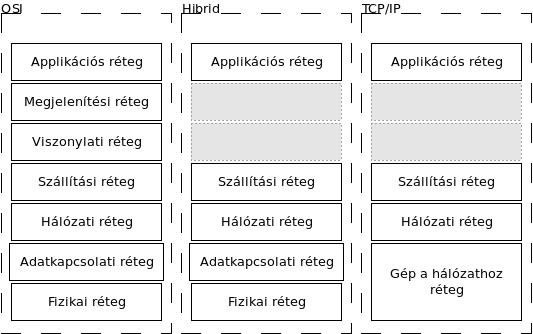
\includegraphics[width=0.6\linewidth]{fig/7-Models}
	\caption{A három modell összehasonlítása}
	\label{fig:7-models}
\end{figure}

A TCP/IP tervezői úgy gondolták, hogy az alkalmazási rétegnek magába kell foglalnia az OSI viszonyrétegének és megjelenítési rétegének részleteit is. Így az általuk létrehozott alkalmazási réteg a megjelenítés, a kódolás és a párbeszédvezérlés kérdéseit kezeli. 

A szállítási réteg a szolgáltatás minőségi kérdéseivel foglalkozik, vagyis a megbízhatósággal, az adatfolyam-vezérléssel és a hibajavítással. Az egyik ide tartozó protokoll, a Transmission Control Protocol (TCP) igen hatékony és rugalmas módon teszi lehetővé a megbízható, gyors, alacsony hibaarányú hálózati kommunikációt. 

A TCP egy összeköttetés alapú (más néven kapcsolatorientált) protokoll. Ez a protokoll párbeszédszerű kommunikációt tart fenn a forrás- és a célállomás között, és szegmensekbe csomagolja az alkalmazási rétegből származó információkat. A kapcsolatorientáltság nem jelenti azt, hogy áramkör létezik a kommunikáló számítógépek között. Azt jelenti, hogy a két állomás között 4. rétegbeli szegmensek haladnak oda-vissza, nyugtázva, hogy bizonyos időtartamra fennáll a logikai összeköttetés.

Az internet réteg rendeltetése, hogy csomagokra bontsa a TCP-szegmenseket, és elküldje őket bármely hálózatról. A csomagok megérkeznek a célhálózatra, attól függetlenül, hogy milyen útvonalon jutottak el oda. Ennek a rétegnek a feladatát az Internetprotokoll (IP) látja el. A legjobb útvonal kiválasztása és a csomagkapcsolás ebben a rétegben történik.

A hálózat-elérési réteg nevének nagyon tág a jelentése, ezért némileg megtévesztő lehet. Másképpen állomás-hálózat közötti rétegnek is nevezzük. Ebbe a rétegbe tartozik minden olyan fizikai és logikai összetevő, amely a fizikai összeköttetés létrehozásához szükséges. Ide tartoznak a hálózati technológiák részletei, beleértve az OSI modell fizikai és adatkapcsolati rétegének minden részletét.

A leggyakrabban használt alkalmazási rétegbeli protokollok közé tartoznak például a következők: 
\begin{itemize}[nosep]
	\item FTP -- File Transfer Protocol (20-21/tcp)
	\item HTTP -- HyperText Transfer Protocol (80/tcp)
	\item HTTPS -- HyperText Transfer Protocol Secure (443/tcp)
	\item SMTP -- Simple Mail Transfer Protocol (25/tcp)
	\item DHCP -- Dynamic Host Configuration Protocol (67-28/udp)
	\item DNS -- Domain Name System (53/udp,tcp)
	\item SFTP -- Secure File Transfer Protocol (22/tcp)
	\item SSH -- Secure SHell (22/tcp)
\end{itemize}

A szállítási réteg gyakoribb protokolljai:
\begin{itemize}[nosep]
	\item TCP -- Transport Control Protocol
	\item UDP -- User Datagram Protocol
\end{itemize}

Az internet réteg a TCP/IP protokollstruktúra fontosabb protokolljai:
\begin{itemize}[nosep]
	\item IP -- Internet Protocol
	\item ICMP -- Internet Control Message Protocol
\end{itemize}